% Standalone: attacker decision tree P1--P4
\documentclass[tikz,border=6pt]{standalone}
\usepackage{amsmath}
\usetikzlibrary{arrows.meta,positioning,shapes.geometric}
\begin{document}
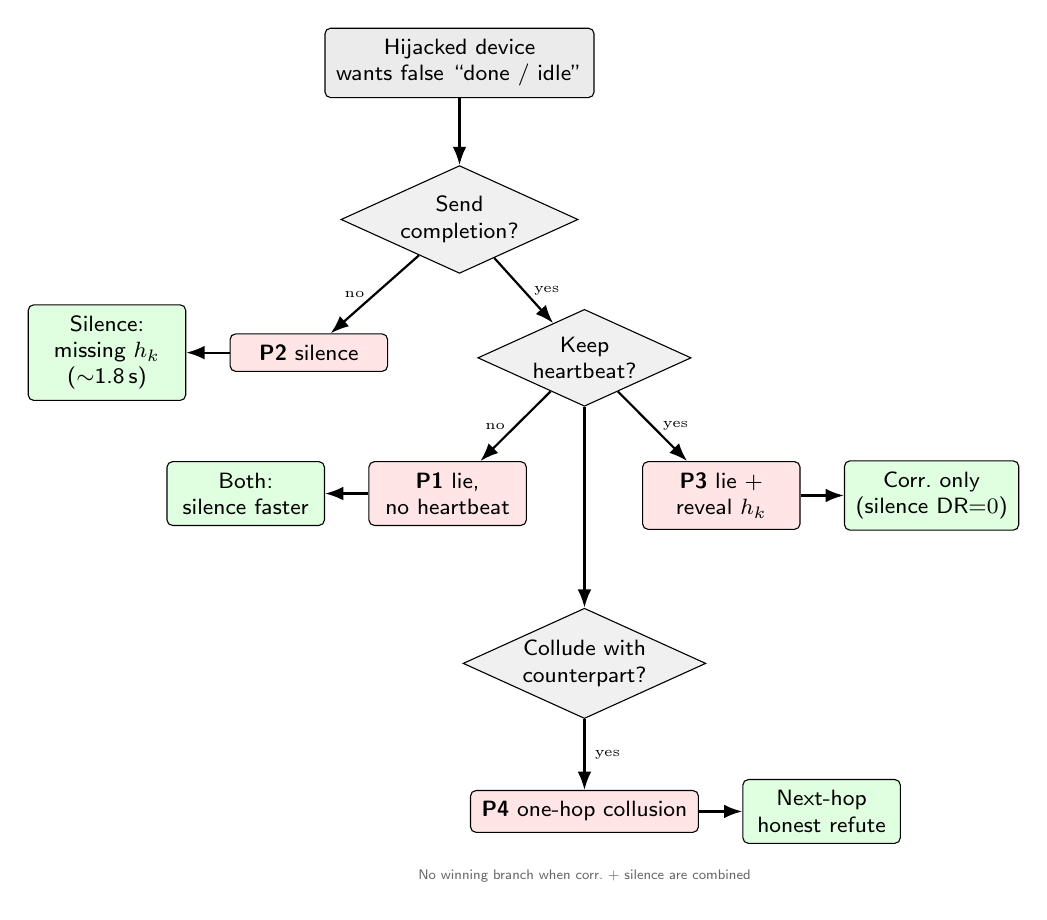
\begin{tikzpicture}[
  font=\sffamily\footnotesize,
  every node/.style={align=center},
  dec/.style={diamond, draw, fill=gray!12, aspect=2.2, inner sep=1pt, minimum width=2.1cm},
  atk/.style={draw, rounded corners=2pt, fill=red!10, inner sep=4pt, minimum width=2.0cm},
  det/.style={draw, rounded corners=2pt, fill=green!12, inner sep=4pt, minimum width=2.0cm},
  fail/.style={draw, rounded corners=2pt, fill=black!8, inner sep=4pt},
  arr/.style={-{Latex}, thick},
]
\node[fail] (root) {Hijacked device\\wants false ``done / idle''};
\node[dec, below=0.85cm of root] (q1) {Send\\completion?};
\node[atk, below left=1.1cm and 0.15cm of q1] (p2) {\textbf{P2} silence};
\node[dec, below right=1.1cm and 0.15cm of q1] (q2) {Keep\\heartbeat?};
\node[atk, below left=1.0cm and 0.05cm of q2] (p1) {\textbf{P1} lie,\\no heartbeat};
\node[atk, below right=1.0cm and 0.05cm of q2] (p3) {\textbf{P3} lie +\\reveal $h_k$};
\node[dec, below=2.55cm of q2] (q3) {Collude with\\counterpart?};
\node[atk, below=0.9cm of q3] (p4) {\textbf{P4} one-hop collusion};

\node[det, left=0.55cm of p2] (d2) {Silence:\\missing $h_k$\\($\sim$1.8\,s)};
\node[det, left=0.55cm of p1] (d1) {Both:\\silence faster};
\node[det, right=0.55cm of p3] (d3) {Corr.\ only\\(silence DR${=}0$)};
\node[det, right=0.55cm of p4] (d4) {Next-hop\\honest refute};

\draw[arr] (root) -- (q1);
\draw[arr] (q1) -- node[left, font=\tiny] {no} (p2);
\draw[arr] (q1) -- node[right, font=\tiny] {yes} (q2);
\draw[arr] (q2) -- node[left, font=\tiny] {no} (p1);
\draw[arr] (q2) -- node[right, font=\tiny] {yes} (p3);
\draw[arr] (q2) -- ++(0,-1.55) -- (q3);
\draw[arr] (q3) -- node[right, font=\tiny] {yes} (p4);
\draw[arr] (p2) -- (d2);
\draw[arr] (p1) -- (d1);
\draw[arr] (p3) -- (d3);
\draw[arr] (p4) -- (d4);

\node[below=0.35cm of p4, font=\sffamily\tiny, text=black!60] {No winning branch when corr.\ + silence are combined};
\end{tikzpicture}
\end{document}
